\section{Notebook in bioinformatic}
\subsection*{Literate programming}

\begin{frame}
What is literate programming ?

\emph{
"Let us change our traditional attitude to the construction of programs: \\
Instead of imagining that our main task is to instruct a computer what to do, let us concentrate rather on explaining to humans what we want the computer to do."}
\footnote{Donald E. Knuth, Literate Programming, 1984} 
\newline
\emph{
”Literate programming is a programming paradigm introduced by Donald Knuth in
which a computer program is given an explanation of its logic in a natural language,
such as English, interspersed with snippets of macros and traditional source code,
from which compilable source code can be generated.”}
\footnote{\url{https://en.wikipedia.org/wiki/Literate_programming\# Workflow}}
\end{frame}

\begin{frame}{Literate programming}
Why using literate programming frameworks ?
\begin{itemize}
	\item Labbook
	\item Day-to-day analysis
	\item Make automatic reports
	\item Write scientific article
\end{itemize}
\end{frame}

\begin{frame}{Literate programming}{example}
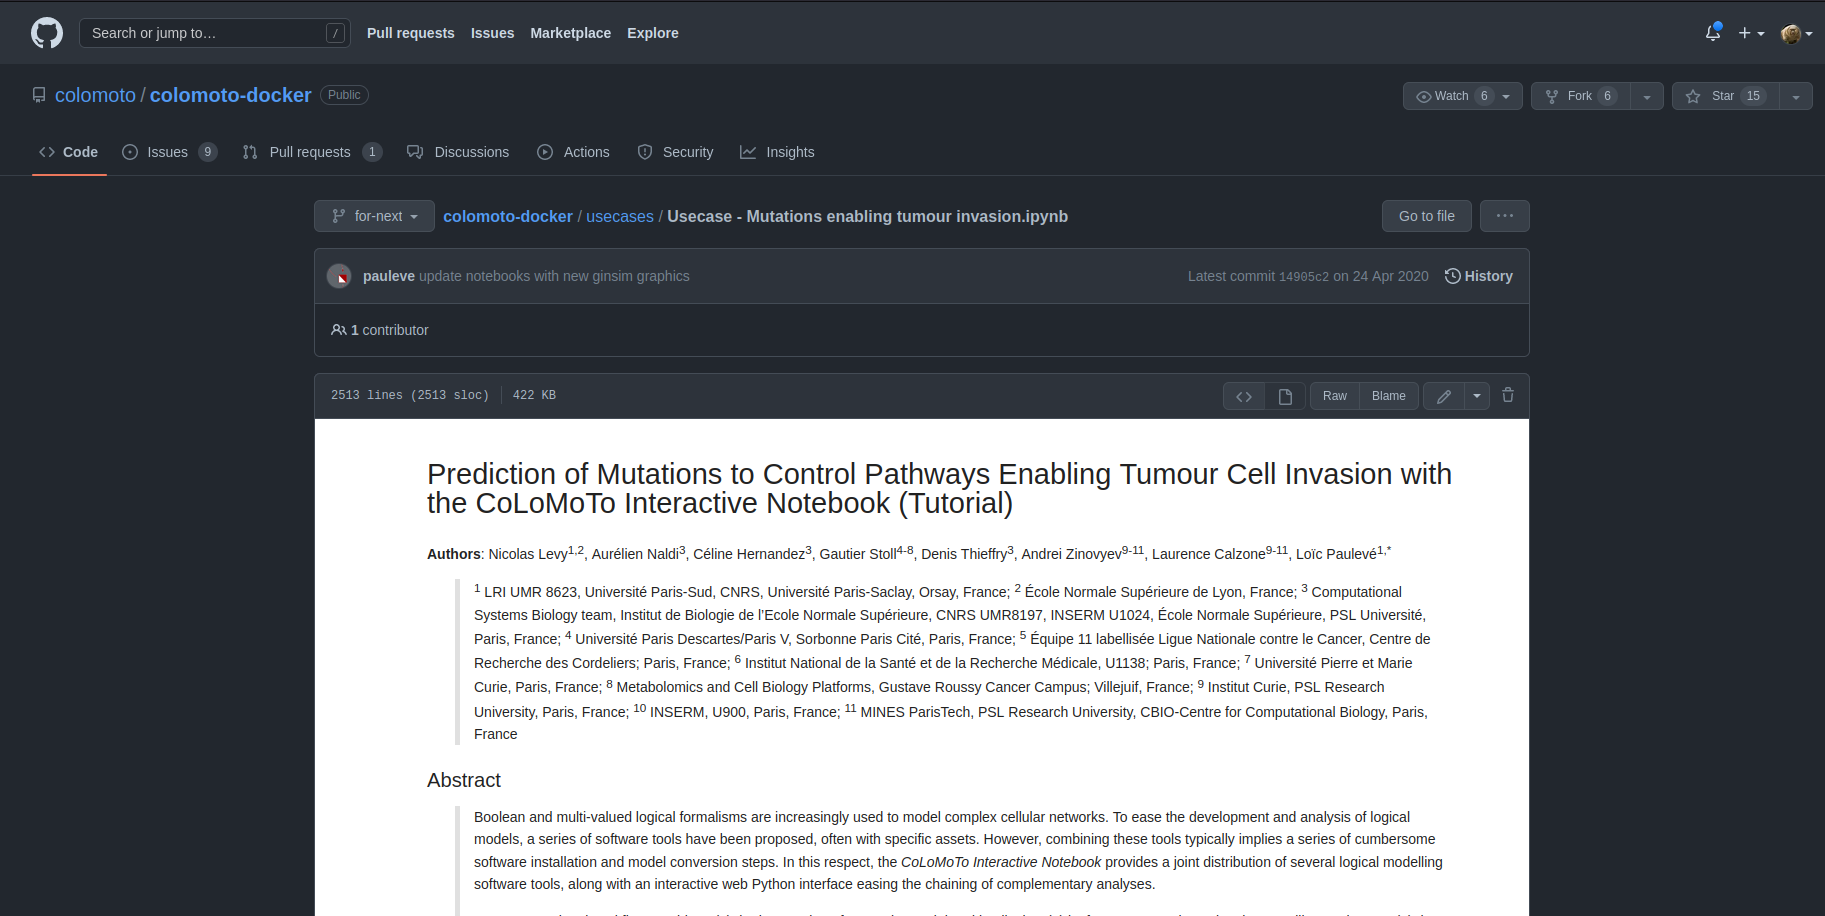
\includegraphics[width=2.3cm,height=1.3cm]{images/colomoto_github.png}
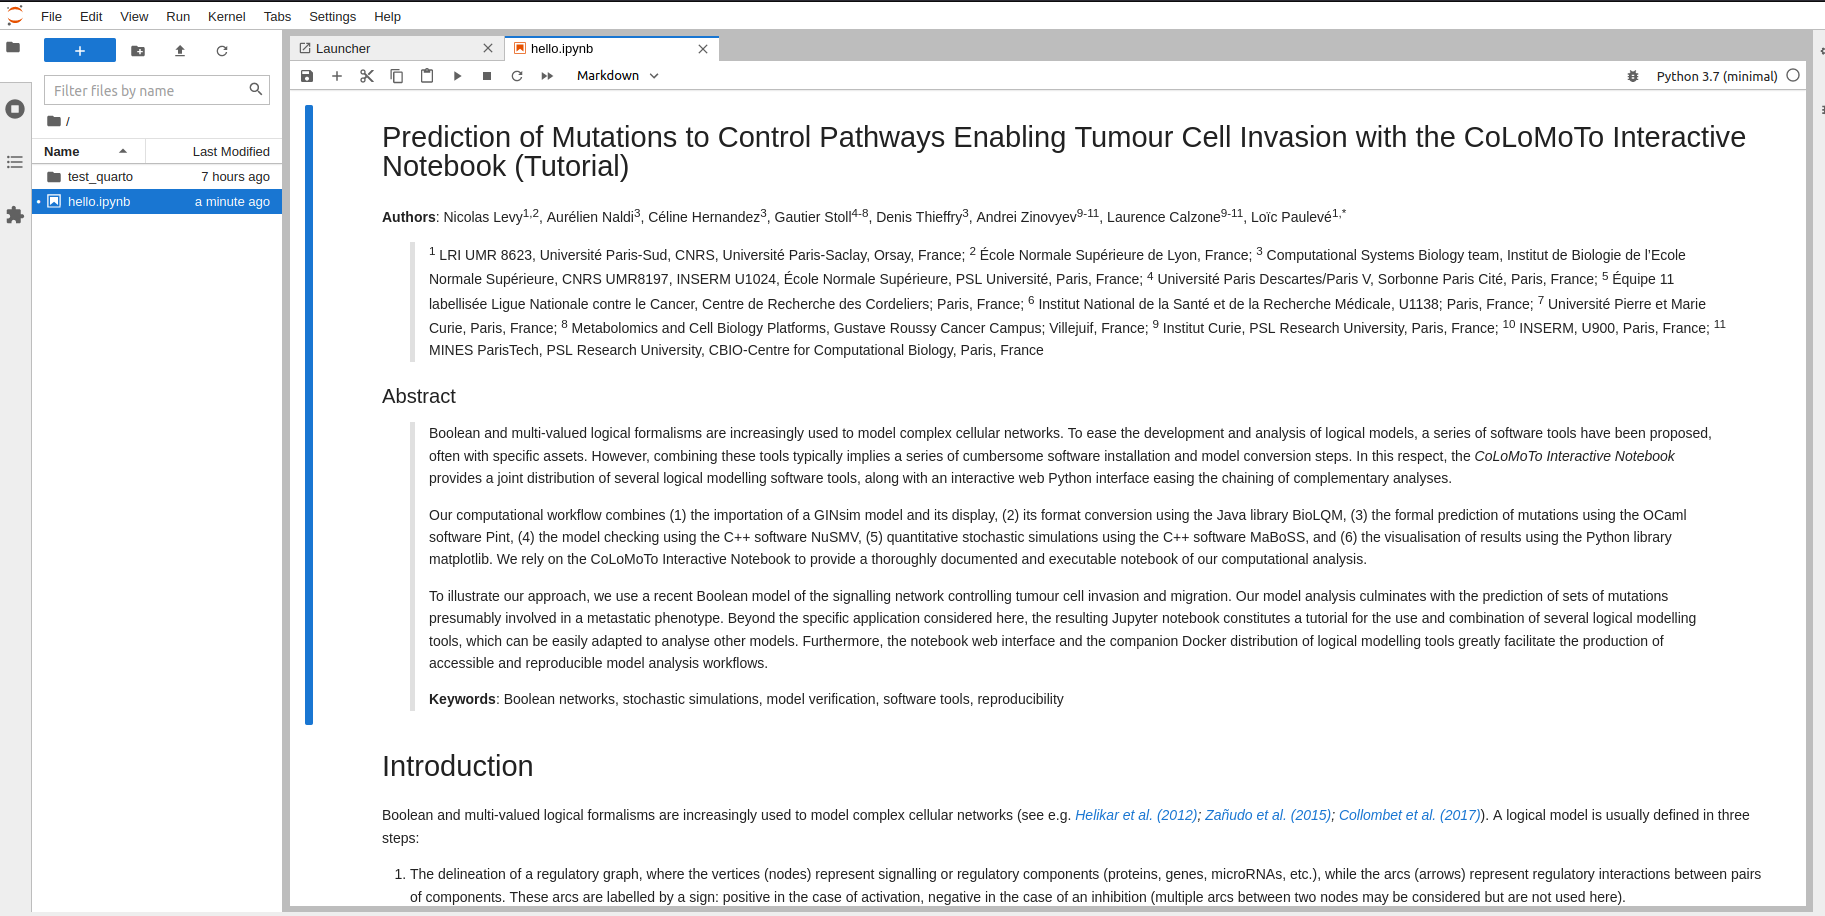
\includegraphics[width=2.3cm,height=1.3cm]{images/colomoto_jupyter.png}
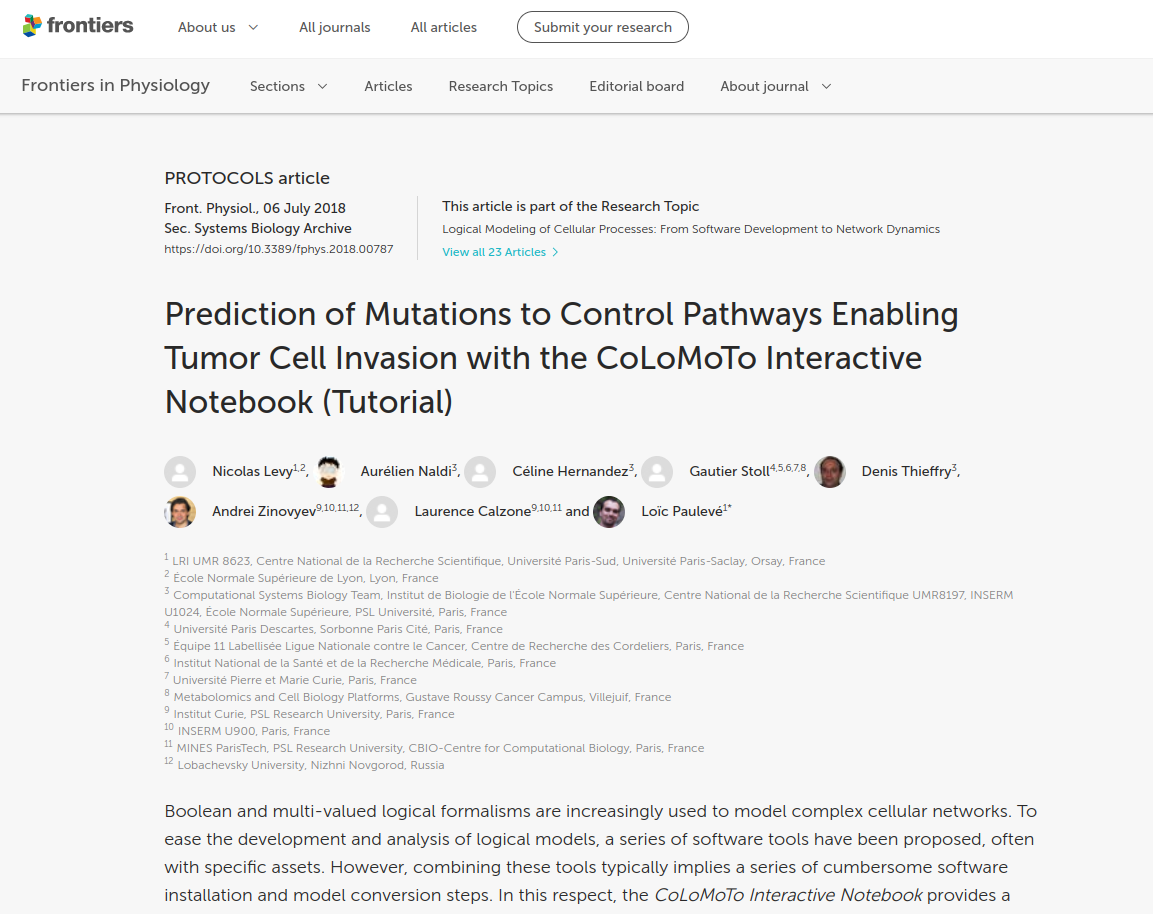
\includegraphics[width=2.3cm,height=1.3cm]{images/colomoto_paper.png}
\href{https://www.frontiersin.org/articles/10.3389/fphys.2018.00787/full}{doi:10.3389/fphys.2018.00787}
\end{frame}

\section{Notebook in bioinformatic}
\subsection*{Literate programming}